\FILE{usecase/hvac.tex}
\subsection{Use Case: HVAC Recommendation}

\TODO{??}{move to authors: Olivera Kotevska, Research Scientist, Oak Ridge National Laboratory, U.S.A.}

\paragraph*{Background.}

Continuous streaming data is produced by heat ventilation and air conditioning (HVAC) systems every
day from the residential houses. This data is stored in a databased on the cloud as it arrives. The data
is used to calculate what should be the next HVAC set point in the house with respect to user
preferences. Periodic recommendations considering environmental parameters, user comfort level
and past user preferences require advanced machine learning algorithm called reinforcement
learning \footnote{this sentence needs grammar edit. Accurate recommendations can save energy and reduce cost. This functionality has three
parts Environmental Forecasting (EF), Learning from the past, (LP), and Set-Point Recommendation
(SPR). EF calculates weather temperature and price predictions. LP learns from the behavior in the
past. SPR model calculates next set-point based on past experience and EF predictions. Figure \ref{fig:hvac-1} shows
the general modeling system flow chat.

\begin{figure}[htb]
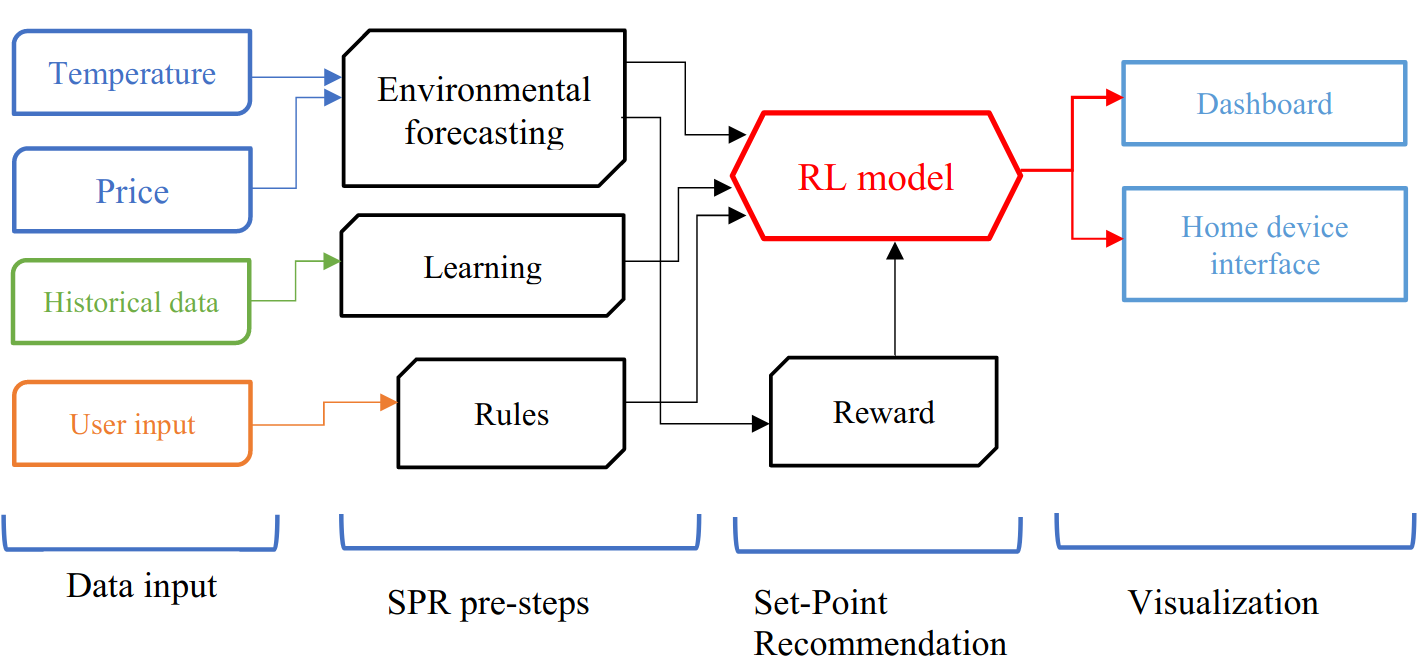
\includegraphics[width=1.0\textwidth]{usecase/hvac.png}
\label{fig:hvac-1}
\caption{HVAC general modeling system flow chat.}
\end{figure}


\paragraph*{Functionalities and Activities} (based on Big Data Application Provider of NBDIF Ref. Architecture).


In this case study, we only focus on three main functionalities, namely EF, LP and SPR, and their
activities. Figure \ref{fig:hvac-2} shows the cross-functional diagram for their actions.



\begin{figure}[htb]
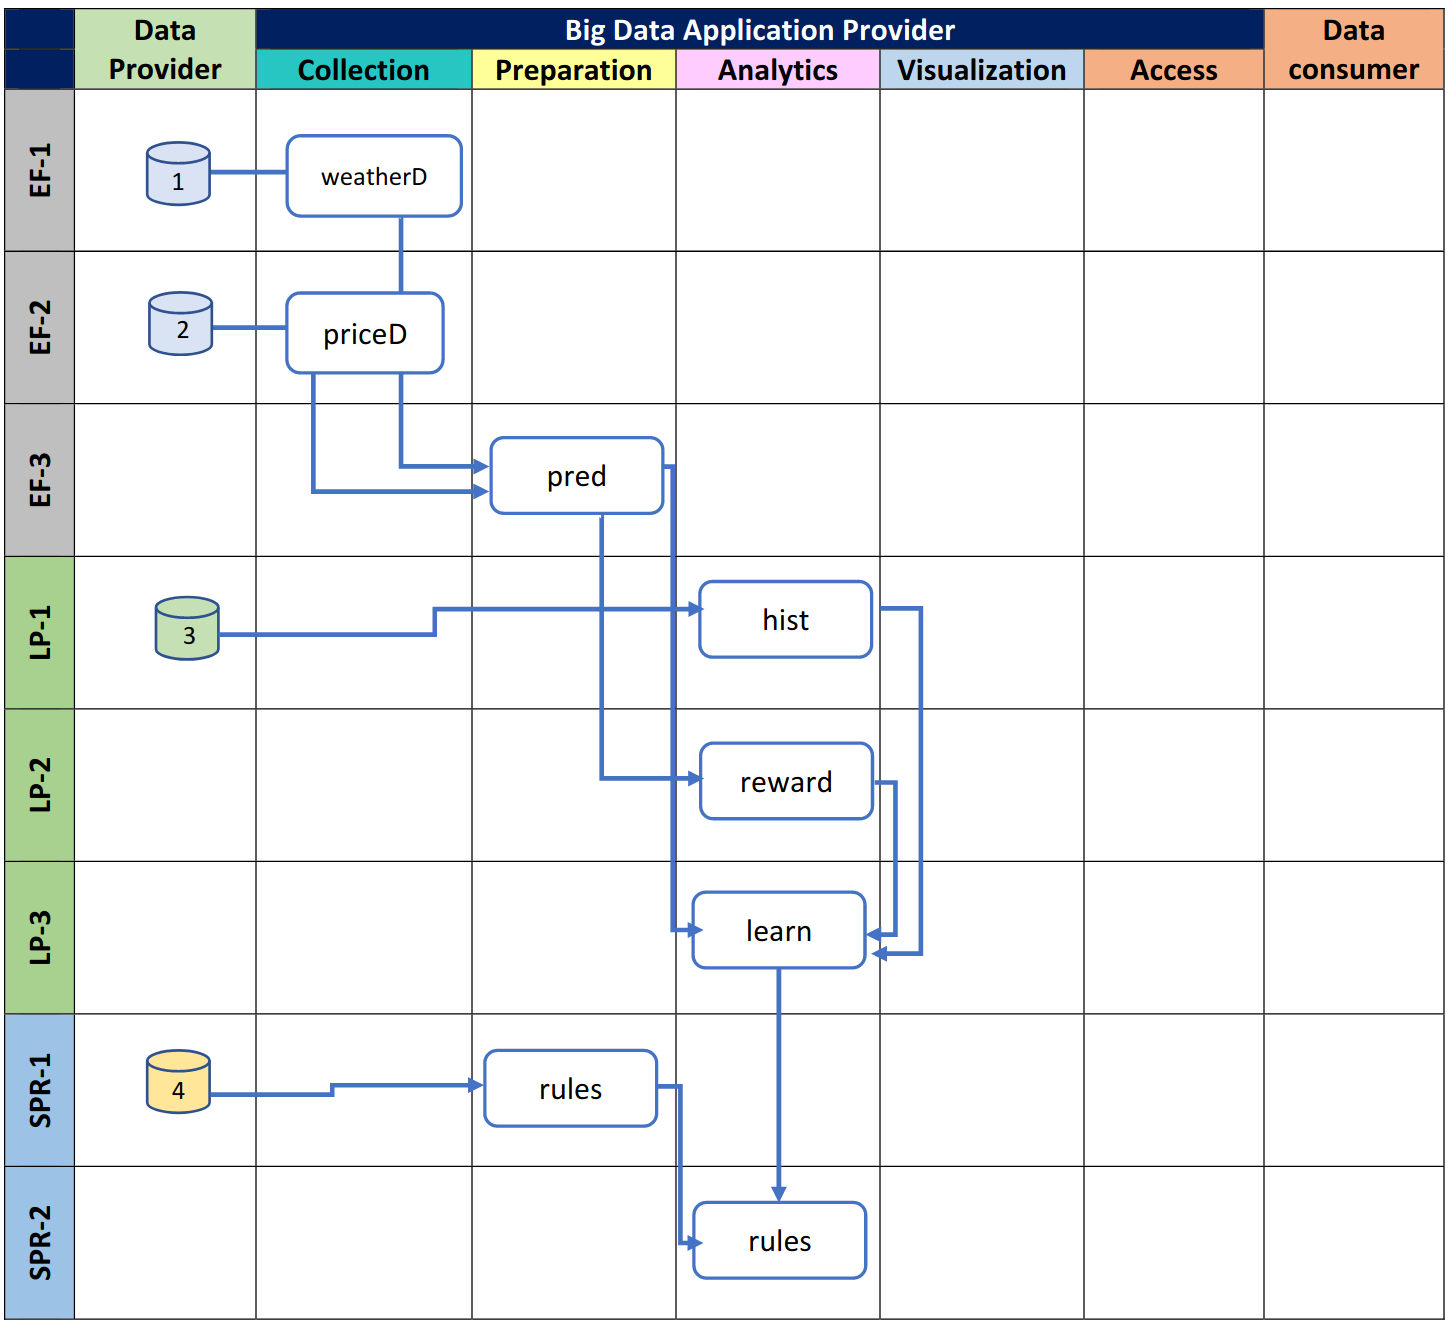
\includegraphics[width=1.0\textwidth]{usecase/hvac-2.png}
\label{fig:hvac-2}
\caption{Cross-Functional Diagram HVAC Recommendation.}
\end{figure}


EF Activities:

\begin{enumerate}
\item weatherD – Collects current weather temperature and predicted temperature for timestamp
X.
\item priceD – Collects current electricity price and predicted price for timestamp X.
\item pred – Extract needed data fields and packs it into an intermediate file format. Input data
from the output of weatherD and priceD.
\end{enumerate}


LP Activities:

\begin{enumerate}
\item hist – Prepares history data points and creates initial condition weights.
\item reward – Generates reward based on the current weatherD and priceD.
\item learn – Collects data from current weatherD, priced, reward.
\end{enumerate}

SPR Activities:

\begin{enumerate}
\item rules – Creates rules based on user preferences and conversion preferences.
\item rlmodel – Interpolates the output from learn, rules and generates set point recommendation
\end{enumerate}

\TODO{??}{No datasets provided.}
